\documentclass[12pt, a4paper]{memoir} % for a short document
\usepackage[french,english]{babel}

\usepackage [vscale=0.76,includehead]{geometry}                % See geometry.pdf to learn the layout options. There are lots.
%\geometry{a4paper}                   % ... or a4paper or a5paper or ...
%\geometry{landscape}                % Activate for for rotated page geometry
%\OnehalfSpacing
% \setSingleSpace{1.05}
%\usepackage[parfill]{parskip}    % Activate to begin paragraphs with an empty line rather than an indent


%===================================== packages
\usepackage{lipsum}
\usepackage{graphicx}
\usepackage{amsmath}
\usepackage{fullpage}
\usepackage{mathptmx} % font = times
\usepackage{helvet} % font sf = helvetica
\usepackage[latin1]{inputenc}
\usepackage{relsize}
\usepackage[T1]{fontenc}
\usepackage{tikz}
\usepackage{booktabs}
\usepackage{textcomp}%textquotesingle
\usepackage{multirow}
\usepackage{pgfplots}
\usepackage{url}
\usepackage{footnote}
%============================================
\usetikzlibrary{arrows,shapes,positioning,shadows,trees}
\makesavenoteenv{tabular}
\makesavenoteenv{table}
%==============================================
\def\checkmark{\tikz\fill[scale=0.4](0,.35) -- (.25,0) -- (1,.7) -- (.25,.15) -- cycle;}
%Style des têtes de section, headings, chapitre
\headstyles{komalike}
\nouppercaseheads
\chapterstyle{dash}
\makeevenhead{headings}{\sffamily\thepage}{}{\sffamily\leftmark}
\makeoddhead{headings}{\sffamily\rightmark}{}{\sffamily\thepage}
\makeoddfoot{plain}{}{}{} % Pages chapitre.
\makeheadrule{headings}{\textwidth}{\normalrulethickness}
%\renewcommand{\leftmark}{\thechapter ---}
\renewcommand{\chaptername}{\relax}
\renewcommand{\chaptitlefont}{ \sffamily\bfseries \LARGE}
\renewcommand{\chapnumfont}{ \sffamily\bfseries \LARGE}
\setsecnumdepth{subsection}


% Title page formatting -- do not change!
\pretitle{\HUGE\sffamily \bfseries\begin{center}}
\posttitle{\end{center}}
\preauthor{\LARGE  \sffamily \bfseries\begin{center}}
\postauthor{\par\end{center}}
\newcommand{\jury}[1]{%
\gdef\juryB{#1}}
\newcommand{\juryB}{}
\newcommand{\session}[1]{%
\gdef\sessionB{#1}}
\newcommand{\sessionB}{}
\newcommand{\option}[1]{%
\gdef\optionB{#1}}
\newcommand{\optionB} {}

\renewcommand{\maketitlehookd}{%
\vfill{}  \large\par\noindent
\begin{center}\juryB \bigskip\sessionB\end{center}
\vspace{-1.5cm}}
\renewcommand{\maketitlehooka}{%
\vspace{-1.5cm}\noindent
\includegraphics[height=12ex]{pics/logo-uga.png}\hfill\raisebox{2ex}{
\includegraphics[height=14ex]{pics/logoINP.png}}\\
\bigskip
\begin{center} \large
Master of Science in Informatics at Grenoble \\
Master Informatique \\
Specialization \optionB  \end{center}\vfill}
% =======================End of title page formatting

\option{Type your Option Here}
\title{Your Title} %\\\vspace{-1ex}\rule{10ex}{0.5pt} \\sub-title}
\author{Your Name}
\date{Defense Date, 2017} % Delete this line to display the current date
\jury{
Research project performed at YOUR LAB \\\medskip
Under the supervision of:\\
Your Supervisor\\\medskip
Defended before a jury composed of:\\
Head of the jury\\
Jury member 1\\
Jury member 2\\
}
\session{Month \hfill 2017}
\setcounter{tocdepth}{4}
\setcounter{secnumdepth}{4}

%%% BEGIN DOCUMENT
\begin{document}
\selectlanguage{English} % french si rapport en français
\frontmatter
\begin{titlingpage}
\maketitle
\end{titlingpage}

%\small
\setlength{\parskip}{-1pt plus 1pt}

\renewcommand{\abstracttextfont}{\normalfont}
\abstractintoc
\begin{abstract}
Your abstract goes here...
\end{abstract}
\abstractintoc

\renewcommand\abstractname{Acknowledgement}
\begin{abstract}
I would like to express my sincere gratitude to .. for his invaluable assistance and comments in reviewing this report...
Good luck :)
\end{abstract}


\renewcommand\abstractname{R\'esum\'e}
\begin{abstract} \selectlanguage{French}
Your abstract in French goes here...
\end{abstract}
\selectlanguage{English}

\cleardoublepage

\tableofcontents* % the asterisk means that the table of contents itself isn't put into the ToC
\normalsize

\mainmatter
\SingleSpace
%==============================CHAPTERS==================
\chapter{Introduction}


\section{Background}

\section{Problem Statement}

A part of the computer graphics is create non-photorealistic images. A method to do this is to stylize 3D objects and 3D scenes. Stylize an object means create an image that imitates the style of an artist who would have drawn it on sheet of paper. There exist many different styles like hand drawing, brush painting, pointillism painting, stippling, watercolor painting, etc.

The main problem of stylizing a 3D object in an animation is the \textit{temporal coherence}. The \textit{temporal coherence} problem in non-photorealistic rendering encompasses both spatial and temporal aspects of the marks. The effect given by the stylization has to be kept if the object is moving, rotating and scaling. Many research has been done to solve this problem of \textit{temporal coherence} \cite{vergne_implicit_2011, benard_dynamic_2009, bleron_motion-coherent_2018}. Bénard et al. separate this problem is three sections inspired by previous work\cite{meier_painterly_1996, cunzi_dynamic_nodate, breslav_dynamic_nodate, benard_state---art_2011} the ideal solution (Figure \ref{problem_temporal_coherence} a) could correspond to something drawn by an artist at each frame. Neglect one of this three goals provide artifacts (Figure \ref{problem_temporal_coherence} b-d).

\begin{figure}
    \begin{center}
    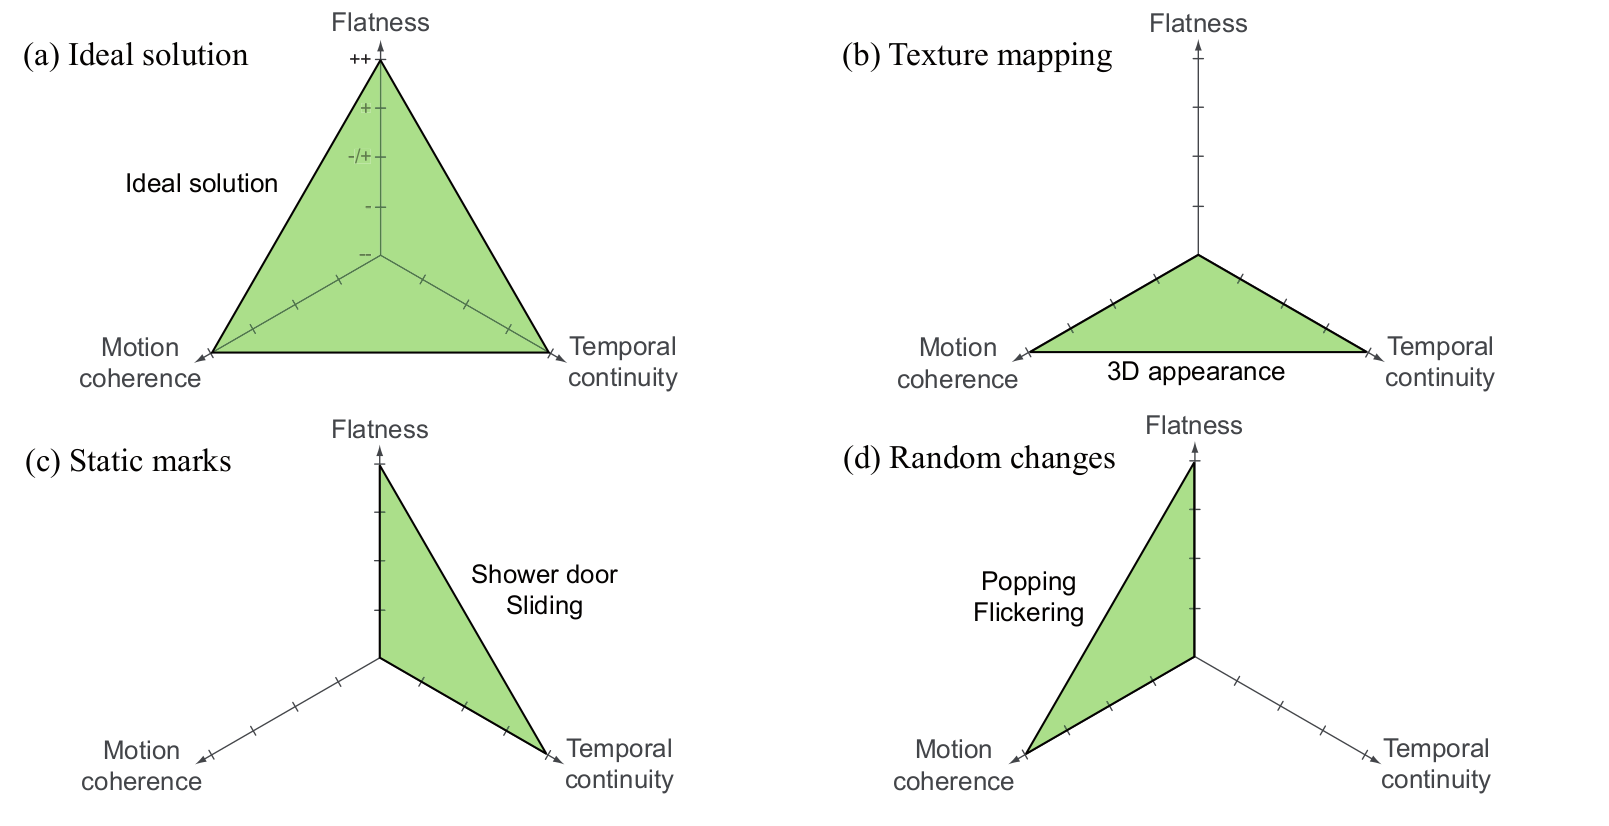
\includegraphics[scale=0.3]{pics/temporal_coherence.png}
    \end{center}
    \caption{Problem involve by temporal coherence depending of the flatness, temporal continuity, motion coherence.}
    \label{problem_temporal_coherence}
\end{figure}

\subsection{Flatness}

The impression of drawing on a flat surface gives the \textit{flatness}. The stylization has a good \textit{flatness} if the image rendered has a good 2D appearance. In order to keep this effect, the size and the distribution of the marks of your stylization have to be independent of the distance between the stylized object and the camera.

\subsection{Motion Coherence}

\textit{Motion coherence} is a correlation between the motion of marks and the motion of the 3D object. Bad \textit{Motion coherence} will give the impression to see the scene through a semi-transparent layer of marks, this is called \textit{shower door} effect \cite{meier_painterly_1996}, an example to illustrate what happens when there is a bad \textit{Motion coherence} is the movie \textit{Loving Vincent}\cite{LovingVincent}. The goal is to provide in 2D screen space a perceptual impression of motion as
close as possible to the 3D displacement in object space.

\subsection{Temporal continuity}

\textit{Temporal continuity} is the quality of minimizing changes from frame to frame to ensure fluid animations. In order to have good \textit{temporal continuity}, the marks of the image have to fade slowly during the animation. Human perception is very sensitive to \textit{temporal incoherence} according to some perceptual studies\cite{percept_studies, Schwarz_2009}. \newline


The problem introduced in the works of Bénard et al.\cite{benard_state---art_2011} is the difficulty to have a ideal solution, the one that has a good \textit{flatness}, a good \textit{motion coherence} and a good \textit{temporal continuity}. These three goals are inherently contradictory when you improve one you neglect one or maybe more. So researchers work to find solutions that make \textit{trade-offs} between these three goals. Our solution is a \textit{trade-offs} too.

\section{Scientific approach}

\section{Contents of this report}

\chapter{Previous Work}



The problem of stylizing a 3D object has received many attention in previous work. There are many methods to stylize. Each of these method have their advantages and disadvantages about the temporal coherence. We separated these ways to stylized in four differents sections.


\section{Image Space}

This simpliest way to stylize a 3D model is to do in image space. The scene is rendered as an image in a texture and from this image the stylization can proceed.
The idea is from this image succeed to compute at each pixel the right color of the splat if this is stroke based rendering or which color of an external texture have to be put on this pixel.
To do an initial painting with strokes Hertzmann's [Image and Video-Based Artistic Stylisation, 2013] add strokes colored depending on the image in the image and decide to delete or replace it to fit at best curves to edges of the image.
Implicit Brushes for Stylized Line-based Rendering [R.Vergne, 2011] use convolution of points to have an hand drawing effect. These points are placed depending on the \textit{feature profile} which is extracted from the image using maximum of the luminance gradient and the DeCarlo algorithm.
\section{Object Space}

\section{Texture Mapping}

\section{Stroke Based}

\chapter{Conclusion}





\subsection{Futur works}

\appendix \chapter{Appendix} 

Appendix goes here...
%=========================================================


%=========================================================
\backmatter

\bibliographystyle{plain} % plain-fr si rapport en français
\bibliography{bibfile.bib}

%\cleardoublepage % Goes to an odd page
%\pagestyle{empty} % no page number
%~\newpage % goes to a new even page

\end{document}
